\begin{minipage}{0.75\linewidth}
\begin{figure}[h]
    \centering
    \begin{adjustbox}{max width=1.0\linewidth, keepaspectratio}
        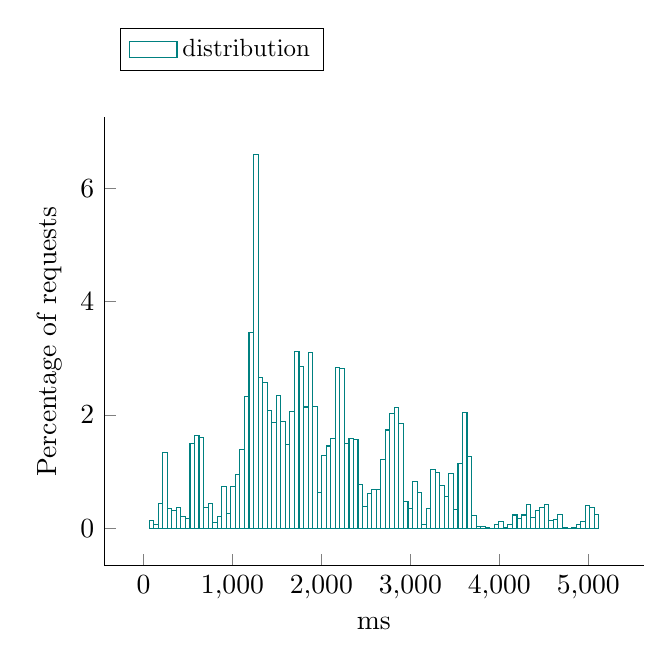
\begin{tikzpicture}
            \begin{axis}[ylabel = Percentage of requests, 
xlabel = ms, 
legend style = {nodes={scale=0.9, transform shape}, at={(0.03,1.2)}, anchor=north west, draw=black, fill=white, align=left, legend columns=3},
area style, mark size = 0pt,
 cycle list name = exotic,
  axis lines* = left]
		\addplot +[ybar interval] coordinates {
			 (63, 0.140625)
			 (114.06, 0.0625)
			 (165.12, 0.4375)
			 (216.18, 1.34375)
			 (267.24, 0.34375)
			 (318.3, 0.3125)
			 (369.36, 0.359375)
			 (420.42, 0.203125)
			 (471.48, 0.171875)
			 (522.54, 1.5)
			 (573.6, 1.64062)
			 (624.66, 1.60938)
			 (675.72, 0.359375)
			 (726.78, 0.4375)
			 (777.84, 0.109375)
			 (828.9, 0.203125)
			 (879.96, 0.734375)
			 (931.02, 0.265625)
			 (982.08, 0.734375)
			 (1033.14, 0.953125)
			 (1084.2, 1.39062)
			 (1135.26, 2.32812)
			 (1186.32, 3.45312)
			 (1237.38, 6.59375)
			 (1288.44, 2.65625)
			 (1339.5, 2.57812)
			 (1390.56, 2.07812)
			 (1441.62, 1.875)
			 (1492.68, 2.34375)
			 (1543.74, 1.89062)
			 (1594.8, 1.48438)
			 (1645.86, 2.0625)
			 (1696.92, 3.125)
			 (1747.98, 2.85938)
			 (1799.04, 2.14062)
			 (1850.1, 3.10938)
			 (1901.16, 2.15625)
			 (1952.22, 0.625)
			 (2003.28, 1.28125)
			 (2054.34, 1.45312)
			 (2105.4, 1.57812)
			 (2156.46, 2.84375)
			 (2207.52, 2.8125)
			 (2258.58, 1.5)
			 (2309.64, 1.57812)
			 (2360.7, 1.5625)
			 (2411.76, 0.765625)
			 (2462.82, 0.390625)
			 (2513.88, 0.609375)
			 (2564.94, 0.6875)
			 (2616, 0.6875)
			 (2667.06, 1.21875)
			 (2718.12, 1.73438)
			 (2769.18, 2.03125)
			 (2820.24, 2.125)
			 (2871.3, 1.84375)
			 (2922.36, 0.46875)
			 (2973.42, 0.34375)
			 (3024.48, 0.828125)
			 (3075.54, 0.625)
			 (3126.6, 0.0625)
			 (3177.66, 0.34375)
			 (3228.72, 1.03125)
			 (3279.78, 0.984375)
			 (3330.84, 0.75)
			 (3381.9, 0.5625)
			 (3432.96, 0.96875)
			 (3484.02, 0.328125)
			 (3535.08, 1.14062)
			 (3586.14, 2.04688)
			 (3637.2, 1.26562)
			 (3688.26, 0.21875)
			 (3739.32, 0.03125)
			 (3790.38, 0.03125)
			 (3841.44, 0.015625)
			 (3892.5, 0)
			 (3943.56, 0.0625)
			 (3994.62, 0.125)
			 (4045.68, 0.015625)
			 (4096.74, 0.0625)
			 (4147.8, 0.234375)
			 (4198.86, 0.171875)
			 (4249.92, 0.234375)
			 (4300.98, 0.421875)
			 (4352.04, 0.1875)
			 (4403.1, 0.3125)
			 (4454.16, 0.359375)
			 (4505.22, 0.421875)
			 (4556.28, 0.140625)
			 (4607.34, 0.15625)
			 (4658.4, 0.25)
			 (4709.46, 0.015625)
			 (4760.52, 0)
			 (4811.58, 0.015625)
			 (4862.64, 0.0625)
			 (4913.7, 0.125)
			 (4964.76, 0.40625)
			 (5015.82, 0.359375)
			 (5066.88, 0.25)
			 (5117.94, 0.171875)
		};
\addlegendentry{distribution};
           \end{axis}
      \end{tikzpicture}
  \end{adjustbox}
  \caption{Response time distribution - req = ReadTimeline-3}
\end{figure}
\end{minipage}\hfill\begin{minipage}{0.18\linewidth}
\begin{table}[h]
\begin{tabular}{|cc|}
\hline
\textbf{} & \textbf{ms}\\ \hline
 \Xhline{0.005\arrayrulewidth}
min & 63\\
 \Xhline{0.005\arrayrulewidth}
max & 5169\\
 \Xhline{0.005\arrayrulewidth}
mean & 2020\\
 \Xhline{0.005\arrayrulewidth}
std & 1002\\
\hline
\hline
 \Xhline{0.005\arrayrulewidth}
25th & 1280\\
 \Xhline{0.005\arrayrulewidth}
50th & 1839\\
 \Xhline{0.005\arrayrulewidth}
75th & 2691\\
 \Xhline{0.005\arrayrulewidth}
80th & 2834\\
 \Xhline{0.005\arrayrulewidth}
85th & 3075\\
 \Xhline{0.005\arrayrulewidth}
90th & 3469\\
 \Xhline{0.005\arrayrulewidth}
95th & 3682\\
 \Xhline{0.005\arrayrulewidth}
99th & 4992\\
\hline
\end{tabular}
\caption{Response time}
\end{table}
\end{minipage}\hfill